\documentclass[12pt]{beamer}
\usetheme{metropolis}
\newenvironment{code}{\ttfamily}{\par}
\title{Where does \textit{your} compiler come from?}
\date{2018-03-13}
\author{Vincent Ambo}
\institute{Norwegian Unix User Group}
\begin{document}
  \maketitle

  %% Slide 1:
  \section{Introduction}


  %% Slide 2:
  \begin{frame}{Chicken and egg}
    Self-hosted compilers are often built using themselves, for example:

    \begin{itemize}
    \item C-family compilers bootstrap themselves \& each other
    \item (Some!) Common Lisp compilers can bootstrap each other
    \item \texttt{rustc} bootstraps itself with a previous version
    \item ... same for many other languages!
    \end{itemize}
  \end{frame}

  %% Slide 3:
  \begin{frame}{Trusting Trust}
    \begin{center}
      Could this be exploited?
    \end{center}
  \end{frame}

  %% Slide 4:
  \begin{frame}{Short interlude: A quine}
    \begin{center}
      \begin{code}
        ((lambda (x) (list x (list 'quote x)))
        \newline\vspace*{6mm} '(lambda (x) (list x (list 'quote x))))
      \end{code}
    \end{center}
  \end{frame}

  %% Slide 5:
  \begin{frame}{Short interlude: Quine Relay}
    \begin{center}
      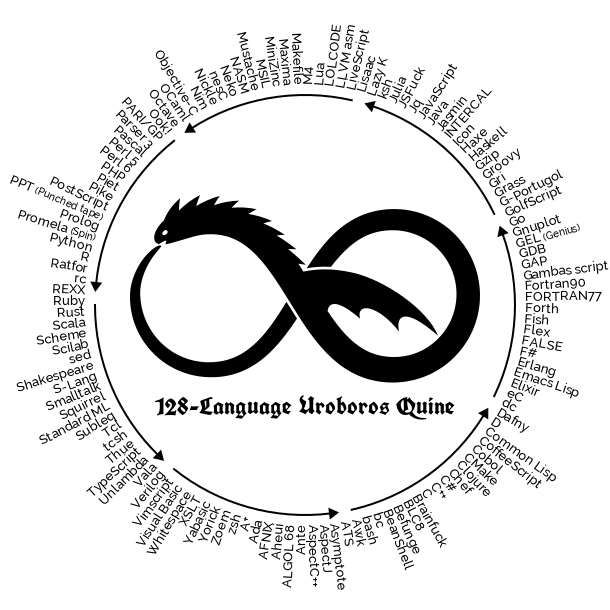
\includegraphics[
        keepaspectratio=true,
        height=\textheight
      ]{quine-relay.png}
    \end{center}
  \end{frame}

  %% Slide 6:
  \begin{frame}{Trusting Trust}
    An attack described by Ken Thompson in 1984:

    \begin{enumerate}
    \item Modify a compiler to detect when it's compiling itself.
    \item Let the modification insert \textit{itself} into the new compiler.
    \item Add arbitrary attack code to the modification.
    \end{enumerate}
  \end{frame}

  %% Slide 7:
  \begin{frame}{Damage potential?}
    \begin{center}
      Let your imagination run wild!
    \end{center}
  \end{frame}

  %% Slide 8:
  \section{Countermeasures}

  %% Slide 9:
  \begin{frame}{Diverse Double-Compiling}
    Assume we have:

    \begin{itemize}
    \item Target language compilers $A$ and $T$
    \item The source code of $A$: $ S_{A} $
    \end{itemize}
  \end{frame}

  %% Slide 10:
  \begin{frame}{Diverse Double-Compiling}
    Apply the first stage (functional equivalence):

    \begin{itemize}
    \item $ X = A(S_{A})$
    \item $ Y = T(S_{A})$
    \end{itemize}

    Apply the second stage (bit-for-bit equivalence):

    \begin{itemize}
    \item $ V = X(S_{A})$
    \item $ W = Y(S_{A})$
    \end{itemize}

    Now we have a new problem: Reproducibility!
  \end{frame}

  %% Slide 11:
  \begin{frame}{Reproducibility}
    Bit-for-bit equivalent output is hard, for example:

    \begin{itemize}
    \item Timestamps in output artifacts
    \item Non-deterministic linking order in concurrent builds
    \item Non-deterministic VM \& memory states in outputs
    \item Randomness in builds (sic!)
    \end{itemize}
  \end{frame}

  %% Slide 12:
  \section{(Partial) State of the Union}

  \begin{frame}{Bootstrapping Debian}

  \end{frame}

  \begin{frame}{Bootstrapping NixOS}

  \end{frame}

  \section{The future of bootstrapping}

  \begin{frame}{MES}
  \end{frame}

  \begin{frame}{The Nix project(s)}
  \end{frame}

  \begin{frame}{Other platforms}

  \end{frame}
  %% Next up: Debian, Fedora, NixOS
  %% Next up: Relevant projects: Nix, MES
  %% Next up: There's hope, but don't even think about phones ...
\end{document}
